\documentclass[bachelor, och, labwork]{shiza}

\usepackage[utf8]{inputenc}
\usepackage{graphicx}

\usepackage[sort,compress]{cite}
\usepackage{amsmath}
\usepackage{amssymb}
\usepackage{amsthm}
\usepackage{fancyvrb}
\usepackage{longtable}
\usepackage{array}
\usepackage[english,russian]{babel}
\usepackage{minted}

\usepackage{tempora}


% \usepackage[colorlinks=false]{hyperref}


\newcommand{\eqdef}{\stackrel {\rm def}{=}}


\begin{document}

\title{Алгоритмы алгебры и теории чисел}

\course{4}

\group{431}

\napravlenie{10.05.01 "--- Компьютерная безопасность}


\author{Никитина Арсения Владимировича}


\satitle{доцент}
\saname{А.\,С.\,Гераськин}


\date{2022}

\maketitle

% Включение нумерации рисунков, формул и таблиц по разделам
% (по умолчанию - нумерация сквозная)
% (допускается оба вида нумерации)
%\secNumbering


\tableofcontents

\section{Задание лабораторной работы}

Разложение полиномов на свободные от квадратов множители:

\begin{itemize}
    \item Алгоритм разложения на свободные от квадратов множители
\end{itemize}

\section{Теоретическая часть}

\begin{center}
    \textit{Разложение полиномов на свободные от квадратов мно-
множители (Polynomial Squarefree Factorization)}
\end{center}

\textit{Вход:} $p_(x)$ --- примитивный полином положительной степени
от одной переменной над областью $J$ характеристики нуль с
однозначным разложением на множители.

\textit{Выход:} Полиномы $s_i(x)$ и число $e$, такие, что $p(x) = \prod_{i=1}^{e} [s_i(x)]^i$ ---
разложение полинома $p(x)$ на свободные от квадратов множители.

\begin{enumerate}
   \item Инициализировать $r(x) := \mathtt{gcd}[p(x), p^{'}(x)], ~ t:= p(x)/r(x), ~j:=1$
   \item Если $deg[r(x)] = 0$, то ответ --- $e = j, ~s_j(x)=t(x)$.
   \item Вычислить $s_j$: $v(x) := \mathtt{gcd}[r(x), t(x)], ~ s_j := t(x)/v(x)$.
   \item $r(x)$ присвоить значение $r(x)/v(x)$, $t(x)$ присвоить значение $v(x)$,
   $j:= j + 1$. Перейти к шагу 2. 
\end{enumerate}


\section{Практическая часть}
\subsection{Пример работы алгоритма}
\begin{figure}[H]
    \centering
    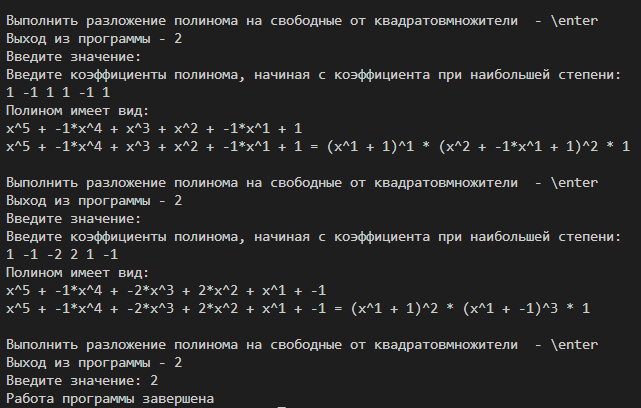
\includegraphics[width=1\textwidth]{pic1.png}
    \caption{}
\end{figure}


\setminted[python]{linenos,breaklines=true, fontsize=\small, style=bw}
    \subsection{Код программы, реализующей рассмотренный алгоритм}
        \inputminted{python}{lab17.py}


\end{document}